%auto-ignore
%      this ensures the arxiv doesn't try to start TeXing here.
%!TEX root = super_lattice_models_draft.tex
%      prev line helps TeXShop do the right thing


%%%%%%%%%%%%%%%%%%%%%%%%%%%%%%%%%%%
\section{Fermion condensation in $SO(3)_6$} \label{so36}
%%%%%%%%%%%%%%%%%%%%%%%%%%%%%%%%%%%

Here we provide more examples of fermion condensation in two theories which are closely related to each other:
$SU(2)_6$ and $SO(3)_6$. 
Each theory contains a fermion $\psi$, which we will condense. 
The main difference between these two theories is that in $SO(3)_6$ the fermion $\psi$ is transparent 
(i.e.\ it braids trivially with every other particle in the theory), while in $SU(2)_6$ it is not. 
This means that when condensing $\psi$ in $SO(3)_6$, we do not need to use the ``back wall'' construction employed earlier,
and the quotient theory will be braided. 
However, the transparency of $\psi$ also means that the $S$-matrix in the $SO(3)_6$ theory is degenerate, 
and hence the theory is not modular. 
In this case the lack of modularity is fairly benign, 
$SO(3)_6$ is a subcategory of the modular tensor category $SU(2)_6$.
This will allow us to infer the minimal idempotents of $SO(3)_6/\psi$ from the minimal idempotents of $SU(2)_6/\psi$.
From the minimal idempotents one can also compute the mapping class group action, which we will work out for the $SO(3)_6/\psi$ example.
First we will establish some notation for UBFC's with fermions.




%%%%%%%%%%%%%%%%%%%%%%%%%%%%%%%%%
\subsection{Fusion theory of $SU(2)_6/\psi$ and $SO(3)_6/\psi$}
%%%%%%%%%%%%%%%%%%%%%%%%%%%%%%%%%

We will now briefly review $SU(2)_6$ and its connection with $SO(3)_6$.
Since these are well known theories we only list out some of their key properties and point the 
reader to some references for more details: see e.g. \cite{kirillow1989} and \cite{Bonderson2007}.
There are seven objects in $SU(2)_6$, labeled by $0,1,2,\cdots, 6$.
The principle graph for the theory is shown in the upper left of Fig.~\ref{SUSOsix}. 
The $0$ particle is the trivial object, $6$ is a fermion, and we have $6 \tp x = (6-x)$. 
Hence the particle $3$ is invariant under fusion with $6$, and so under condensation of the $6$ 
particle $3$ becomes a q-type simple object in $SU(2)_6/\psi$.
Since one m-type particle is always related to another by fusion with $\psi$ and 
there are six m-type particles, there are only three distinct equivalence classes of m-type
particles under fusion with $\psi$. 
We can take $\{0,1,2\}$ as the complete list of representatives.

We give the principle graph for $SU(2)_6/\psi$ in Fig.~\ref{SUSOsix} in the upper right, where $q_3$ is the q-type image of $3$ under condensation.
\begin{figure} 
\centering
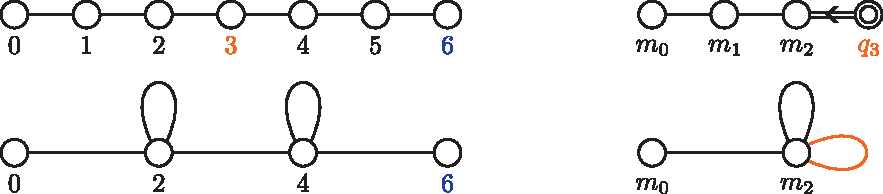
\includegraphics{SU26SO36Dynkin.pdf}
\caption{\label{SUSOsix} The upper left diagram is the principle graph of $SU(2)_6$, and the 
lower left diagram is the principle graph for $SO(3)_6$. 
On the right we give the principle graphs of the condensed theories $SU(2)_6/\psi$ (top right) and 
$SO(3)_6/\psi$ (bottom right), both with the identification $\psi=6$. 
The naming convention of the condensed theories has been inherited from the parent theories, 
along with an $m$ or $q$ denoting whether the particle is m-type or q-type.
Black links denote even fusion channels, and the red link connecting $m_2$ to itself 
denotes an odd fusion channel in accordance with the rule $m_2\tp m_2 \cong m_0 \oplus \cc^{1|1}m_2$. 
}
\end{figure}
The particles $0,2,4,$ and $6$ form a closed sub-category of $SU(2)_6$. 
The principle graph of this theory is shown in the bottom left of Fig.~\ref{SUSOsix}. 
This is the subcategory known as $SO(3)_6$, it is a braided theory, with braiding and 
fusion inherited from $SU(2)_6$, however, it is not modular.
The $6$ particle braids trivially within this subcategory, and is therefore transparent, 
which breaks the modularity.

We now perform fermion condensation in $SU(2)_6$ and $SO(3)_6$ to obtain two super pivotal 
categories $SU(2)_6/\psi$ and $SO(3)_6/\psi$. 
Since $\psi$ is not transparent in $SU(2)_6$, we must perform the back-wall condensation 
process described earlier. 
However, since $\psi$ {\it is} transparent in $SO(3)_6$, condensation of $\psi$ is possible 
without employing a back-wall (although a spin structure is still needed). 
The principle graphs of the condensed theories are shown on the right of Fig.~\ref{SUSOsix}.
The simple objects of the two theories are given as follows:
\begin{align}
\xymatrix @!0 @M=1mm @C=10mm {
SU(2)_6/\psi:&&m_0 & m_1 & m_2 & q_3 \\
SO(3)_6/ \psi:&&m_0 && m_2& 
}
\end{align}
The particles have a natural grading given by (\ref{grading}) with the even set given by 
$I_0 = \{ m_0, m_2 \}$ and the odd set given by $I_1 = \{m_1, q_3\}$, with $I_a \tp I_b = I_{a+b \;  \text{mod} \; 2}$.
The closed sub-fusion algebra given by $I_0$ contains all of the objects in $SO(3)_6/\psi$, 
which occurs since $\psi$ is transparent in $SO(3)_6$. 
Note that there are no q-type objects in $SO(3)_6/\psi$. 

The non-trivial fusion rules of $SU(2)_6/\psi$ are given in Table \ref{SU2six_psi_fusion}.
\begin{table} 
\begin{align}
\xymatrix{
\text{
{\tabulinesep=1.2mm
\begin{tabu}{ c | c c  c c |c  c   }
$I_0 \tp I_0$&$m_0$ &$m_2$&$\quad\quad$&
$I_0 \tp I_1$&$m_1 $& $q_3$\\  
\cline{1-3}\cline{5-7}$m_0$&$m_0$ & $m_2$ &&
$m_0$& $m_1 $& $q_3$\\   
$m_2$ & $m_2$ & $m_0 \oplus \mathbb{C}^{1|1}m_2$&&
$m_2$ &$ m_1\oplus q_3 $ & $\mathbb{C}^{1|1} m_1 \oplus q_3$\\
\multicolumn{1}{r}{}&& &&\multicolumn{1}{r}{}&&\\
$I_1 \tp I_0$&$m_0 $& $m_2$ &&
$I_1 \tp I_1$ &$m_1 $& $q_3$\\  
\cline{1-3}\cline{5-7} $m_1$& $m_1 $& $m_1\oplus q_3$ &&
$m_1$ &$m_0 \oplus m_2$&$ \mathbb{C}^{1|1} m_2$ \\
$q_3$ &$ q_3  $ & $\mathbb{C}^{1|1} m_1 \oplus q_3$ &&
$q_3$ &$\mathbb{C}^{1|1} m_2 $&$ \mathbb{C}^{1|1}m_0 \oplus \mathbb{C}^{1|1}m_2$\\
\end{tabu}
}}
}
\end{align}
\caption{Fusion rules for $SU(2)_6/\psi$
\label{SU2six_psi_fusion}}
\end{table}

We note two features of these examples which were not present in our earlier $C_2$ example:
\begin{itemize}
\item Even though $m_2$ is an m-type particle, $\mathbb{C}^{1|1}m_2$ 
appears in the tensor product of $m_2$ with itself.
So $SO(3)_6/\psi$ provides us with an example of a theory which has 
no q-type objects, but which is still fermionic in the sense that its fusion spaces contain both even and odd elements. 
\item The q-type particle $q_3$ appears in the tensor product of two m-type 
particles, namely $m_2 \tp m_1$. 
Thus the classification of simple objects as m- or q-type should not be thought of as a $\zz/2$ grading, since the types of 
$a$ and $b$ in no way constrain the possible types of the simple objects appearing in $a\tp b$.
(In the next section we will also see an example of two q-type particles fusing to another q-type particle.)
\end{itemize}


The $F$-symbols of the condensed theories can be deduced from those of the parent theories, so we will not list them here.
We now compute the minimal idempotents of the tube category in the condensed theories.


%%%%%%%%%%%%%%%%%%%%%%%%%%%
\subsection{Primitive idempotents of $SU(2)_6/\psi$}
\label{SU2psiIdempotents}
%%%%%%%%%%%%%%%%%%%%%%%%%%%

The primitive idempotents of the tube category of $SU(2)_6/\psi$ can be computed directly 
using the techniques of Section \ref{more_on_tubes}. 
They are given by
\begin{align}
E(a,b) = \TubeIdempotentTwoStrandab_{J}, \quad \quad  (a,b) \in \sob(SU(2)_6) \times \sob(SU(2)_6/\psi),
\end{align}
where as before we require that $s(J) = (-1)^{\nu_b}$.
It will be useful to recast these idempotents in a form 
that can be easily used to compute the idempotents for $SO(3)_6$. 
We first define
\begin{align}
\widetilde{E}(a,b,\cl(r)) \; = \; \BasisForIdempotents
\end{align}
and for $x = \unit$ or $x = \psi$ we define the $\omega_x$ loop 
\begin{align}
 \omega_x = \frac{d_x}{\mathcal{D}_{\mcc/\psi}^2} \sum_{r\in \sob(\mcc/\psi)} \frac{d_r }{ \dim\End(r)} \left( \frac{S_{xr}}{S_{\unit r}} \right)   \cl(r).
\end{align}
The $S$-matrix above is that of the parent theory, and the labels are trivial lifts from $\mcc/\psi$.
When $x = \unit$, $ \frac{S_{x r}}{S_{\unit r}}=1$ this is just the standard $\omega$ loop, 
when $x =\psi$, $ \frac{S_{x r}}{S_{\unit r}}=(-1)^{\nu_r}$ and $\omega_\psi$ is a projector onto the $\psi$ strand.
The factor $\mcd_{\mcc/\psi}^2 = \sum_{x \in \mcc/\psi} d_x^2 / \dim \End(x)$ is the total quantum dimension of 
the condensed theory in the sense of \eqref{total_qdim_defn}. 
The minimal idempotents given by $E(a,b)$ in \eqref{FunctorCxCtoTubeC}
can be re-written as
\begin{align}
\label{Etilde}
E(a\tp x, b) \cong \widetilde{E}(a,b, \omega_x),
\end{align}
with $a,b \in \mcc/\psi$ and $x =\unit, \psi$.
The isomorphism relating the two idempotents is an odd isomorphism if $x = \psi$.
Notice that running over all all pairs $a,b \in \mcc/\psi$ and $x = \unit$ or $\psi$ runs over all possible $E(a,b)$.
Additionally if $a \tp \psi \cong a$ then $\widetilde{E}(a,b, \omega_\unit)$ and $\widetilde{E}(a,b, \omega_\psi)$ are equivalent. 
This presentation of the idempotents is more symmetric than those discussed in Section \ref{more_on_tubes}.

We now write these idempotents so that they have a single strand at the boundary rather than two.
We use the fermionic analogue of \eqref{TwoStrandToOneStrand}
to write down the single strand idempotents
\begin{align}
\label{OneStrandIdempotent}
\tilde{e}_{ab}(\omega_x,c,j) \; = \; \OneStrandIdempotentMTCpsi.
\end{align}
These idempotents are similar to the ones described earlier in \eqref{idempotent_one_strand}. 
The particular representative of the isomorphism class is given by choosing $c \in a\tp b$, 
and appropriately normalized vectors $\mu_j \in V^{ab}_c(\mcc/\psi)$, and $\nu_j \in V^{c}_{ab}(\mcc/\psi)$.
We will denote the parity of $\mu_j \in V^{ab}_c(\mcc/\psi)$ by $\sigma_j=1$ $(\sigma_j = -1)$ 
if the chosen basis vector $\mu_j$ in the fusion space $V^{ab}_c(\mcc/\psi)$ is even (odd).
The twists of the idempotents are given by 
\begin{align} 
\label{CmodPsiTwistsModular}
T\cdot \tilde{e}(a,b,\omega_x,c,j)  =
\begin{cases} 
  \frac{\theta_a}{\theta_b} (-1)^{x (\nu_a + \nu_b)}\sigma_j\;  \tilde{e}(a,b,\omega_x,c,j) & \text{if bounding}\\[.5em]
\frac{\theta_a}{\theta_b} (-1)^{x (\nu_a + \nu_b)} \; \tilde{e}(a,b,\omega_x,c,j) 
& \text{if non-bounding} \end{cases} 
\end{align} 
We will write $\tilde{e}(a,b,\omega_x,c,j)$ as $m_{ab}(\omega_x,c,j)$ 
if the idempotent is m-type and $q_{ab}(\omega_x,c,j)$ if the idempotent is q-type.
For $SU(2)_6/\psi$ we list a complete set of representatives of minimal idempotents.
We find 14 m-type idempotents for the bounding spin structure, 
and 14 idempotents for the non-bounding spin structure, 7 are m-type and 7 are q-type. 
Explicitly, the idempotents and corresponding twists are listed in tables \ref{bounding_SU26} and \ref{nonbounding_SU26}.
Note that if $a$ is q-type, then $\tilde{e}(a,b,\omega_\unit,j)$ is isomorphic to $\tilde{e}(a,b,\omega_\psi,j)$ and so we only list one of them.
We now turn our attention to the $SO(3)_6$ theory. 
\begin{table}
\begin{center}
\begin{align}
\nonumber
\xymatrix @M=0mm @R=5mm @C=5mm {
&\text{
\begin{tabu}{ c | c }
type& $\quad$twist $\quad$ \\ \hline
$m_{00}(\omega_0,c,j)$ &$1$ \\
$m_{10}(\omega_0,c,j)$ &$e^{3 i \pi /16}$ \\
$m_{20}(\omega_0,c,j)$ &$i$ \\
\end{tabu}
}
&
\text{
\begin{tabu}{ c | c }
type& $\quad$twist $\quad$  \\ \hline
$m_{00}(\omega_\psi,c,j)$ &$1$ \\
$m_{10}(\omega_\psi,c,j)$ &$-e^{3 i \pi/16}$ \\
$m_{20}(\omega_\psi,c,j)$ &$i$ \\
\end{tabu}
}
&
\text{
\begin{tabu}{ c | c }
type& twist $\times \; \sigma_j$ \\ \hline
$m_{30}(\omega_0,c,j)$ &$ e^{15i \pi /16}$ \\
$m_{32}(\omega_0,c,j)$ &$-ie^{15i \pi /16}$ \\
\end{tabu}
}
\\
&\text{
\begin{tabu}{ c | c }
type& twist $\times \; \sigma_j $ \\ \hline
$m_{02}(\omega_0,c,j)$ &$-i $ \\
$m_{12}(\omega_0,c,j)$ &$-i e^{3 i \pi/16}$ \\
$m_{22}(\omega_0,c,j)$ &$1$ \\
\end{tabu}
}
&
\text{
\begin{tabu}{ c | c }
type&twist $\times \; \sigma_j $ \\ \hline
$m_{02}(\omega_\psi,c,j)$ &$-i$ \\
$m_{12}(\omega_\psi,c,j)$ &$ie^{3 i \pi /16}$ \\
$m_{22}(\omega_\psi,c,j)$ &$1$ \\
\end{tabu}
}&}
\end{align}
\caption{ Bounding idempotents for $SU(2)_6/\psi$.
Where $c \in a \tp b$ and $j$ labels the choice of in the fusion space $V^{ab}_c (\mcc/\psi)$.
Some of these labels are determined, 
e.g., $m_{00}(\omega_0,c,j)$ can be simplified to $m_{00}(\omega_0,m_0,0)$.
The pre-factor $\sigma_j$ is $\pm1$ denoting the parity of $\mu_j \in V^{ab}_c$.}
\label{bounding_SU26}
\end{center}
\end{table}

\begin{table}
\begin{center}
\begin{align}
\nonumber
\xymatrix @M=0mm @R=5mm @C=5mm  {
&\text{
\begin{tabu}{ c | c }
type&$\quad  $ twist $\quad \;$ \\ \hline
$m_{01}(\omega_0,c,j)$ &$-e^{-3i\pi/16}$ \\
$m_{11}(\omega_0,c,j)$ &$1$ \\
$m_{21}(\omega_0,c,j)$ &$-i e^{-3i \pi /16}$ \\
\end{tabu}
}
&
\text{
\begin{tabu}{ c | c }
type& $\quad  $ twist $\quad \;$ \\ \hline
$m_{01}(\omega_\psi,c,j)$ &$-e^{-3 i \pi /16}$ \\
$m_{11}(\omega_\psi,c,j)$ &$1$ \\
$m_{21}(\omega_\psi,c,j)$ &$-i e^{-3 i \pi /16}$ \\
\end{tabu}
}
&
\text{
\begin{tabu}{ c | c }
type& twist \\ \hline
$m_{31}(\omega_0,c,j)$ &$e^{3 i \pi /4}$ \\
$q_{33}(\omega_0,c,j)$ &$1$ \\
\end{tabu}
}
\\
&\text{
\begin{tabu}{ c | c }
type& twist \\ \hline
$q_{03}(\omega_0,c,j)$ &$-e^{-15 i \pi /16}$ \\
$q_{13}(\omega_0,c,j)$ &$e^{- 3 i \pi /4}$ \\
$q_{23}(\omega_0,c,j)$ &$-i e^{-15 i \pi /16}$ \\
\end{tabu}
}
&
\text{
\begin{tabu}{ c | c }
type& twist \\ \hline
$q_{03}(\omega_\psi,c,j)$ &$-e^{-15 i \pi /16}$ \\
$q_{13}(\omega_\psi,c,j)$ &$e^{- 3 i \pi /4}$ \\
$q_{23}(\omega_\psi,c,j)$ &$- i e^{- 15i \pi /16}$ \\
\end{tabu}
}&
}
\end{align}
\caption{Non-Bounding idempotents for $SU(2)_6/\psi$
}
\label{nonbounding_SU26}
\end{center}
\end{table}


%%%%%%%%%%%%%%%%%%%%%%%%%%%%%%
\subsection{Primitive idempotents of $SO(3)_6/\psi$}
%%%%%%%%%%%%%%%%%%%%%%%%%%%%%%

Finding the idempotents in the $SO(3)_6/\psi$ theory is more difficult, since the parent theory $SO(3)_6$ isn't modular.
However since $SO(3)_6$ is obtained from $SU(2)_6$ by discarding the elements in $SU(2)_6$ 
that braid nontrivially with $\psi$, $SU(2)_6$ is a modular extension of $SO(3)_6$ (in fact, it is the minimal modular extension). 
This fact will allow us to compute the idempotents in the $SO(3)_6/\psi$ theory using our knowledge of the $SU(2)_6$ theory. 

Applying \eqref{OneStrandIdempotent} directly to $SO(3)_6$ will not yield a complete set of minimal idempotents due to the lack of modularity. 
Instead we use  \eqref{OneStrandIdempotent} by taking pairs of simple objects $(a,b)$ from $SU(2)_6/\psi \times SU(2)_6/\psi$ whose tensor product is in $SO(3)_6/\psi$.
Additionally, within this subset we need to take an appropriate linear combination of the $SU(2)_6/\psi$ idempotents so that the resulting annulus only has strands labeled by objects in $SO(3)_6/\psi$.
This linear combination is given by taking $\tilde{e}_{ab}(\omega_\unit, c,j)+\tilde{e}_{ab}(\omega_\psi, c,j)$ which results in the minimal idempotent
\begin{align}
\widetilde{e}_{ab}( \omega_\unit + \omega_\psi,c,j) \in \tube(SO(3))_6).
\end{align}
where the labels $(a,b) \in I_0/\psi \times I_0/\psi \cup I_1/\psi \times I_1/\psi$.\footnote{
Note that a minimal idempotent of 
$\tube(SO(3)_6/\psi)$ has a trivial lift to an idempotent of $\tube(SU(2)_6/\psi)$ but does not remain minimal.}
One can show that the procedure creates a complete set of minimal idempotents by direct calculation. 
The bounding idempotents are found when $(a,b) \in I_0/\psi \times I_0/\psi$, 
these are the minimal idempotents found from a naive application of \eqref{OneStrandIdempotent}. 
The non-bounding idempotents are given by $(a,b) \in I_1/\psi \times I_1/\psi$



We now write down the minimal idempotents of $SO(3)_6/\psi$ and their twists using the same notation as in Section \ref{SU2psiIdempotents}. 
In the bounding sector $J = B$, we have $4$ m-type idempotents, given by
\begin{align}
\xymatrix{
\text{
{{\tabulinesep=1.2mm
\begin{tabu}{ c c  }
type& twist \\ \hline
$m_{00}(\omega_\unit + \omega_\psi,0,0)$ &$1$ \\
$m_{02}(\omega_\unit + \omega_\psi,2,0)$ &$ -i $\\
$m_{20}(\omega_\unit + \omega_\psi,2,0)$ & $i$\\
$m_{22}(\omega_\unit + \omega_\psi,c,j)$ &$ \sigma_j $\\
\end{tabu}
}}}
} 
\end{align}
with $c \in m_2 \tp m_2$ and $j$ labeling a vector in the fusion space $V^{m_2 m_2}_c(\mcc/\psi)$.
Meanwhile the non-bounding idempotents are given by
\begin{align}
\xymatrix{
\text{
{{\tabulinesep=1.2mm
\begin{tabu}{ c c }
type& twist \\ \hline
$m_{11}(\omega_\unit + \omega_\psi,c,j)$ &$1$ \\
$q_{13}(\omega_\unit + \omega_\psi,2,j)$ &$ e^{-3 i \pi/4} $\\
$q_{31}(\omega_\unit + \omega_\psi,2,j)$ & $e^{3 i \pi /4} $\\
$m_{33}(\omega_\unit + \omega_\psi,c,j)$ &$ 1 $\\
\end{tabu}
}}}
}
\end{align}
Similarly, $c \in m_1 \tp m_1$ and $j$ labels a vector in $V^{m_1 m_1}_c$ for $m_{11}$, 
and $c \in q_3 \tp q_3$ and $j$ labels a vector in $V^{q_3 q_3}_c(\mcc/\psi)$ for $m_{33}$.
Here we've made use of the above observation that only $a \tp b$ need be in $SO(3)_6/\psi$, 
and hence the pairs $(a,b)$ in these idempotents are labeled by $m_1$ and $q_3$.
As the notation suggests $m_{33}$ is not q-type:
 to see this we note that if it were, then there would 
be an odd endomorphism of $\tube(SO(3)_6/\psi)$ with trivial boundary conditions (since $m_0 \in q_3 \tp q_3$).
That would require $SO(3)_6/\psi$ to contain a q-type simple object, 
but as explained in \eqref{noq-type} this is not possible since $\psi$ is transparent in $SO(3)_6$.
One can explicitly construct an odd endomorphism for $q_{13}$ by putting a fermion on $q_3$ and fusing all strands into the annulus;
similarly for $q_{31}$. 


%%%%%%%%%%%%%%%%%%%%%
\subsection{Modular transformations}
\label{SO36ModularTransformations}
%%%%%%%%%%%%%%%%%%%%%

The modular transformations can be computed directly by manipulating string diagrams.
We already have the twists (which are read off from the string-net labels of the idempotents), 
and the modular $T$-transformation can be obtained directly from the twists.
The modular $S$-transformation requires a little more work, 
and so we discuss this in a little more detail.

We first close the minimal idempotents onto the torus. 
Using the basis above, one finds the image under $\text{cl}_Y$ is given by
\begin{align}
\tilde{e}_{ab}(\omega_\unit + \omega_\psi, c, j) \; \xrightarrow{\;\;  \cl_Y \;\;  }\; \tilde{e}_{ab} \;=\;  \TorusBraidBasis{a}{b\;}{}{\omega}{X}{Y}
\end{align}
where $a$ and $b$ label the idempotent as before, $X$ denotes the spin structure of the idempotent which is fixed by $b$, $Y$ denotes the spin structure around the newly closed cycle, 
and $\omega = \omega_\unit + \omega_\psi$. 
Note that when $X$ is non-bounding, 
$a, b\in \{ m_1, q_3 \}$, which lies outside of $SO(3)_6/\psi$.
However, $\tilde{e}_{ab} \in \cl_Y \tube(SO(3)_6/\psi)$ since when the diagram is fused into the torus we find a torus string net labeled with objects only in $SO(3)_6/\psi$, as required.


In this graphical convention, the modular $S$-transformation acts as
\begin{align}
{ \TorusBraidBasis{a}{b\;}{}{\omega}{X}{Y}} \stackrel{S}{\longrightarrow} \sum_{r,w} S^{{XY \rightarrow YX}}_{(a,b),(r,w)} \;
{\TorusBraidBasis{r}{w}{}{\omega}{Y}{X} }\; .
\end{align}
The matrix elements can be computed explicitly using the $S$-matrix of $SU(2)_6$. 
Explicitly, the $S$-matrix acts on each of the three bounding spin tori as 
\begin{align}
\left( \begin{matrix}
m_{00}\\
m_{02}\\
m_{20}\\
m_{22}\\
\end{matrix} \right)_{BB}
\xrightarrow{S^{BB \rightarrow BB}}
\frac{1}{2 \sqrt{2}} \left( \begin{matrix}
\frac{1}{d}&1&1&d \\
1& -\frac{1}{d} & d &-1 \\
1& d& -\frac{1}{d} & -1 \\
d & -1& -1& \frac{1}{d}\\
\end{matrix} \right)
\left( \begin{matrix}
m_{00}\\
m_{02}\\
m_{20}\\
m_{22}\\
\end{matrix} \right)_{BB}
\end{align}

\begin{align}
\left( \begin{matrix}
m_{11}\\
q_{13}\\
q_{31}\\
m_{33}\\
\end{matrix} \right)_{NB}
\xrightarrow{S^{NB \rightarrow BN}}
\frac{1}{2} \left( \begin{matrix}
1&1&1&1\\
1&-1&1&-1\\
1&1&-1&-1\\
1&-1&-1&1\\
\end{matrix} \right)
\left( \begin{matrix}
m_{00}\\
m_{02}\\
m_{20}\\
m_{22}\\
\end{matrix} \right)_{BN}
\end{align}

\begin{align}
\left( \begin{matrix}
m_{00}\\
m_{02}\\
m_{20}\\
m_{22}\\
\end{matrix} \right)_{BN}
\xrightarrow{S^{BN \rightarrow NB}}
\frac{1}{2} \left( \begin{matrix}
1&1&1&1\\
1&-1&1&-1\\
1&1&-1&-1\\
1&-1&-1&1\\
\end{matrix} \right)
\left( \begin{matrix}
m_{11}\\
q_{13}\\
q_{31}\\
m_{33}\\
\end{matrix} \right)_{NB}
\end{align}
As mentioned earlier, 
the Dehn twists follow directly from the twists computed above; 
see \eqref{CmodPsiTwistsModular}.
Again for the bounding spin tori we find
\begin{align}
\left( \begin{matrix}
m_{00}\\
m_{02}\\
m_{20}\\
m_{22}\\
\end{matrix} \right)_{BB}
\xrightarrow{T^{BB \rightarrow BN}}
\left( \begin{matrix}
1&&&\\
&-i&&\\
&&i&\\
&&&1\\
\end{matrix} \right)
\left( \begin{matrix}
m_{00}\\
m_{02}\\
m_{20}\\
m_{22}\\
\end{matrix} \right)_{BN}
\end{align}

\begin{align}
\left( \begin{matrix}
m_{11}\\
q_{13}\\
q_{31}\\
m_{33}\\
\end{matrix} \right)_{NB}
\xrightarrow{T^{NB \rightarrow NB}}
 \left( \begin{matrix}
 1&&&\\
&e^{-3 i \pi /4}&&\\
&&e^{3 i \pi /4}&\\
&&&1\\
\end{matrix} \right)
\left( \begin{matrix}
m_{11}\\
q_{13}\\
q_{31}\\
m_{33}\\
\end{matrix} \right)_{NB}
\end{align}

\begin{align}
\left( \begin{matrix}
m_{00}\\
m_{02}\\
m_{20}\\
m_{22}\\
\end{matrix} \right)_{BN}
\xrightarrow{T^{BN \rightarrow BB}}
\left( \begin{matrix}
1&&&\\
&-i&&\\
&&i&\\
&&&1\\
\end{matrix} \right)
\left( \begin{matrix}
m_{11}\\
q_{13}\\
q_{31}\\
m_{33}\\
\end{matrix} \right)_{BB}
\end{align}
One can verify that $(TS)^3 = \text{id}$, which holds since all three of the spin tori discussed above have 
 even fermion parity (recall that the more general identity is $(ST)^3 = (-1)^F$). 

The modular $S$ transformations on the torus with $NN$ spin structure are a little more tedious to calculate. 
A complete basis 
of net configurations on the $NN$ spin torus is given by
\begin{align}
\underbrace{
\xymatrix{
\TorusBraidBasisd{\scale{.6}{1}}{\scale{.6}{1}\;}{}{\omega}{N}{N}{\TorusBasisMTCNoLabel} \quad 
 \TorusBraidBasisd{\scale{.6}{3} }{\scale{.6}{3} \;}{}{\omega}{N}{N}{\TorusBasisMTCdd}
 \\}
 }_{\text{even}}
 \quad \quad 
\underbrace{
\xymatrix{ \TorusBraidBasisd{\scale{.6}{1}}{\scale{.6}{3}\;}{}{\omega}{N}{N}{\TorusBasisMTCdr} \quad
 \TorusBraidBasisd{\scale{.6}{3} }{\scale{.6}{1} \;}{}{\omega}{N}{N}{\TorusBasisMTCdl}
 \\}
 }_{\text{odd}}
\end{align}
On the non-bounding torus, m-type idempotents always close up into even parity states, 
while q-type idempotents close up into odd parity states.
The first two vectors have even parity and provide a basis for $\cl_N(m_{11})$ and $\cl_N(m_{33})$, 
while the second two have odd parity and provide a basis for $\cl_N(q_{13})$ and $\cl_N(q_{31})$.
After some calculation one finds that the $S$ and $T$ modular matrices act as 
\begin{align}
\left( \begin{matrix}
m_{11}\\
m_{33}\\
\stackrel{\bullet}{q}_{13}\\
\stackrel{\bullet}{q}_{31}\\
\end{matrix} \right)_{NN}
\xrightarrow{S^{NN \rightarrow NN}}
 \left( \begin{matrix}
1&0&&\\
0&1&&\\
&&e^{-i\pi/4}&0\\
&&0&e^{i \pi /4}\\ 
\end{matrix} \right)
\left( \begin{matrix}
m_{11}\\
m_{33}\\
\stackrel{\bullet}{q}_{13}\\
\stackrel{\bullet}{q}_{31}\\
\end{matrix} \right)_{NN}
\end{align}
and 
\begin{align}
\left( \begin{matrix}
m_{11}\\
m_{33}\\
\stackrel{\bullet}{q}_{13}\\
\stackrel{\bullet}{q}_{31}\\
\end{matrix} \right)_{NN}
\xrightarrow{T^{NN \rightarrow NN}}
 \left( \begin{matrix}
1&0&&\\
0&1&&\\
&&e^{-3i\pi/4}&0\\
&&0&e^{3i \pi /4}\\ 
\end{matrix} \right)
\left( \begin{matrix}
m_{11}\\
m_{33}\\
\stackrel{\bullet}{q}_{13}\\
\stackrel{\bullet}{q}_{31}\\
\end{matrix} \right)_{NN}
\end{align}
As required, the odd part of the $S$-matrix satisfies $S^4 = -\text{id}$ and $(TS)^3 = -\text{id}$, 
while the even part satisfies the usual $S^4 = \text{id}$ and $(TS)^3 = \text{id}$. 
